%!TEX TS-program = pdflatex
% paper.tex -- main diss file
%
% Wisconsin dissertation template
% Copyright (c) 2008-2009 William C. Benton.  All rights reserved.
%
% This program can redistributed and/or modified under the terms of the LaTeX
% Project Public License Distributed from CTAN archives in directory
% macros/latex/base/lppl.txt; either version 1 of the License, or (at your
% option) any later version.
%
% This program includes other software that is licensed under the terms of the
% LPPL and the Perl Artistic License; see README for details.
%
% You, the user, still hold the copyright to any document you produce with this
% software (like your dissertation).
%

%%% You'll want ``oneside'' for the deposit version, but probably not for any
%%% versions that don't need to meet the UW requirements
%%% MJG - note that the thesis dept updated the pt requirement from 12 to 10
%%% (2013)
\documentclass[10pt,oneside,letterpaper]{memoir}
\setlrmarginsandblock{1.1in}{*}{1}
\setulmarginsandblock{1.7in}{1in}{*}
\checkandfixthelayout

% preamble.tex -- packages to include
%
% Wisconsin dissertation template
% Copyright (c) 2008 William C. Benton.  All rights reserved.
%
% This program can redistributed and/or modified under the terms
% of the LaTeX Project Public License Distributed from CTAN
% archives in directory macros/latex/base/lppl.txt; either
% version 1 of the License, or (at your option) any later version.
%
% This program includes other software that is licensed under the
% terms of the LPPL and the Perl Artistic License; see README for details.
%
% You, the user, still hold the copyright to any document you produce
% with this software (like your dissertation).

%% Comment out any of these that you don't want
\usepackage{amssymb}
\usepackage{amsmath}
\usepackage{amsthm}
%\usepackage{theorem}
\usepackage{hyperref}

%%%%% LISTINGS package and setup
\IfFileExists{listings.sty}{%
\usepackage{listings}%
}{}

%% Packages added by Matt Gidden
%%
%% Note, order matters!
%%
\usepackage{cite} % right order for multiple entries in cite
\usepackage{moreverb} % for verbatim snippets of code
\usepackage{fancyvrb}
\usepackage{tabularx} % for tables with line breaks
\usepackage{threeparttable} % for tables with notes
\usepackage[capitalize, noabbrev]{cleveref} % for reference multiple figures
\usepackage{calc} % allows for arithmetic on latex variables
\usepackage{float} % allows for figures to be placed explicitly
\usepackage{algorithm2e} % for algorithms
\usepackage{subfig}
\usepackage{multirow} % combining rows in tables
\usepackage{footnote}
\usepackage{titlesec} % for using \titleformat
\usepackage{slashbox} % for tables with a divided cell, see http://tex.stackexchange.com/questions/7262/diagonally-divided-table-cell
\usepackage{bashful}
\usepackage{xspace}
\usepackage{color}
\definecolor{listinggray}{gray}{0.9}
\definecolor{lbcolor}{rgb}{0.9,0.9,0.9}
\lstset{
    %backgroundcolor=\color{lbcolor},
    language={C++},
    tabsize=4,
    rulecolor=\color{black},
    upquote=true,
    aboveskip={1.5\baselineskip},
    belowskip={1.5\baselineskip},
    columns=fixed,
    extendedchars=true,
    breaklines=true,
    prebreak=\raisebox{0ex}[0ex][0ex]{\ensuremath{\hookleftarrow}},
    frame=single,
    showtabs=false,
    showspaces=false,
    showstringspaces=false,
    basicstyle=\scriptsize\ttfamily\color{black},
    keywordstyle=\color[rgb]{0,0,1.0},
    commentstyle=\color[rgb]{0.133,0.545,0.133},
    stringstyle=\color[rgb]{0.627,0.126,0.941},
    numberstyle=\color[rgb]{0,1,0},
    identifierstyle=\color{black},
    captionpos=t,
}
\lstdefinestyle{BashOutputStyle}{
  basicstyle=\small\ttfamily,
  numbers=none,
  frame=tblr,
  columns=fullflexible,
  backgroundcolor=\color{blue!10},
  linewidth=0.9\linewidth,
  xleftmargin=0.1\linewidth
}
%
% Adding for some table features
\usepackage{array}
%
% Adding package for float barriers
\usepackage{placeins}

%% Custom commands added by Matt Gidden
\setcounter{tocdepth}{2}
\setcounter{secnumdepth}{3}
\theoremstyle{plain}
\newcommand{\Cyclopts}{\textsc{Cyclopts} }
\newcommand{\Cycamore}{\textsc{Cycamore} }
\newcommand{\cyclus}{\textsc{Cyclus}\xspace}
\newcommand{\Cyclus}{\textsc{Cyclus} }
\newcommand{\nucl}[2]{
\ensuremath{^{#1}}\mbox{#2}
}
\newcommand{\horizfig}[2][]{%
  \begin{minipage}{3in}\subfloat[#1]{#2}\end{minipage}}
%% \newcommand{\code}[1]{\lstinline[basicstyle=\ttfamily\color{green!40!black}]|#1|}
\newcommand{\code}[1]{\lstinline[basicstyle=\ttfamily\color{black}]|#1|}
\newcommand{\codeb}[1]{\texttt{#1}}
\newcommand{\units}[1] {\:\text{#1}}%
\newcommand{\citeme}{\textcolor{red}{CITE}\xspace}
\newcommand{\TODO}[1] {{\color{red}\textbf{TODO: #1}}}%
\newcommand{\Reactor}[1]{\texttt{Reactor{#1}}}
\newcommand{\UOXSource}{\texttt{UOX\_Source}}
\newcommand{\MOXSource}{\texttt{MOX\_Source}}
\newcommand{\Enrichment}{\texttt{Enrichment}}
\newcommand{\ffc}{$f_{\text{fc}}$\xspace}
\newcommand{\frx}{$f_{\text{rx}}$\xspace}
\newcommand{\floc}{$f_{\text{loc}}$\xspace}
\newcommand{\dloc}{$\delta_{\text{loc}}$\xspace}
\newcommand{\dreg}{$\delta_{\text{reg}}$\xspace}
\newcommand{\cbc}{Cbc\xspace}
\newcommand{\clp}{Clp\xspace}

%% You should use natbib
\IfFileExists{natbib.sty}{%
  \usepackage[numbers]{natbib}% added the numbers option from the original WI
                              % thesis template
}{}

%% You probably need appendix, if you want appendices
\IfFileExists{appendix.sty}{%
\usepackage{appendix}%
}{}

%% the spacing in memoir is weird, you'll need to use this
\DisemulatePackage{setspace}
\usepackage[onehalfspacing]{setspace}

%% List setup; the ``hanglist`` environment will allow you to have
%% nicely-typeset enumerated lists (i.e., with the numbers hanging in
%% the margins).  You need at least version 2.1 of enumitem.sty.  If
%% you don't have enumitem installed at all, hanglist will just be an
%% alias for enumerate.
\IfFileExists{enumitem.sty}{%
\usepackage[loadonly]{enumitem}[2007/06/30]%
\newlist{hanglist}{enumerate}{1}% 
\setlist[hanglist]{label=\arabic*.}%
\setlist[hanglist,1]{leftmargin=0pt}%
}{%
\newenvironment{hanglist}{\begin{enumerate}}{\end{enumerate}}%
}

\IfFileExists{mathpartir.sty}{%
\usepackage{mathpartir}%
}{}

%% \newtheorem{thm}{Theorem}[chapter] % reset theorem numbering for each chapter
%% \theoremstyle{definition}
%% \newtheorem{defn}[thm]{Definition} % definition numbers are dependent on theorem numbers
%% \newtheorem{exmp}[thm]{Example} % same for example numbers


%% Get rid of ugly borders around PDF hyperlinks (e.g., for cross-references, bib entries, or URLs)
\hypersetup{pdfborder = 0 0 0}

%% You want microtype.
\IfFileExists{microtype.sty}{%
\usepackage[protrusion=true,expansion=true]{microtype}%
}{}

%\pagestyle{thesisdraft}

% Surround parts of graphics with box
\usepackage{boxedminipage}

%% booktabs (thx to Nate Rosenblum for bringing this beautiful package
%% to my attention)
\IfFileExists{booktabs.sty}{%
\usepackage{booktabs}%
}{}

% This is now the recommended way for checking for PDFLaTeX:
\usepackage{ifpdf}

%% Avoid ugly "Type 3" fonts
\usepackage{lmodern}
\usepackage[LY1]{fontenc}

%% Substitute your favorite serif and sans fonts here....
\IfFileExists{tgpagella.sty}{%
% TeX Gyre pagella, like Palatino
\usepackage{tgpagella}%
}{}

%% overrides the default Latex math font with AMS Euler
%\usepackage[LY1]{eulervm} 

\ifpdf
\usepackage[pdftex]{graphicx}
\else
\usepackage{graphicx}
\fi

\usepackage{makeidx}
\makeindex

{\theoremstyle{plain}
\newtheorem{thm}{Theorem}[chapter]
\newtheorem{cor}[thm]{Corollary}
\newtheorem{define}[thm]{Definition}
\newtheorem{exmpl}[thm]{Example}
}
{\theoremstyle{remark}
\newtheorem{rmk}[thm]{Remark}
}

\newtheoremstyle{customsty1}
{3pt}%
{3pt}%
{}% --- body font
{}% --- indent amount
{\bfseries}% --- Theorem head font
{:}% --- Punctuation after head
{.5em}% --- space after head
{}% --- theorem head spec (can be left empty, meaning 'normal')

% Define 'newtheorems' that use ``customsty1''
{\theoremstyle{customsty1} 
}


%%% NB: the ``deposit'' chapter- and page- styles should conform to UW
%%% requirements.  If you are producing a pretty version of your
%%% dissertation for web use later, you will certainly want to make
%%% your own chapter and page styles.

\makechapterstyle{deposit}{%
  \renewcommand{\chapterheadstart}{}
  \renewcommand{\printchaptername}{}
  \renewcommand{\chapternamenum}{}
  \renewcommand{\printchapternum}{\parbox{2em}{\MakeLowercase{\Large\scshape\thechapter{}}} }
  \renewcommand{\afterchapternum}{}
  \renewcommand{\printchaptertitle}[1]{%
  \raggedright\Large\scshape\MakeLowercase{##1}}
  \renewcommand{\afterchaptertitle}{%
  \vskip\onelineskip \hrule\vskip\onelineskip}
}

\makepagestyle{deposit}
 
\makeatletter
 
\renewcommand{\chaptermark}[1]{\markboth{#1}{}}
\renewcommand{\sectionmark}[1]{\markboth{#1}{}}
 
\makeevenfoot{deposit}{}{}{}
\makeoddfoot{deposit}{}{}{}
\makeevenhead{deposit}{\thepage}{}{}
\makeoddhead{deposit}{}{}{\thepage}
\makeatother

%%% set up page numbering for chapter pages to satisfy UW requirements
%%% NB: You will want to delete until the ``SNIP'' mark if you are
%%% making a ``nice'' copy
\copypagestyle{chapter}{plain}
\makeoddfoot{chapter}{}{}{}
\makeevenhead{chapter}{\thepage}{}{}
\makeoddhead{chapter}{}{}{\thepage}
%%% SNIP

%%% bib nonsense
\makeatletter
\newenvironment{wb-bib}[1]{%
  \chapter*{references}
\ifnobibintoc\else 
\phantomsection 

\addcontentsline{toc}{chapter}{References } 
\fi 
\prebibhook
  \begin{bibitemlist}{#1}}{\end{bibitemlist}\postbibhook}

\AtBeginDocument{%
  \@ifpackageloaded{natbib}{% natbib is loaded
    \addtodef{\endthebibliography}{}{\vskip-\lastskip\postbibhook}
    \@ifpackagewith{natbib}{sectionbib}{% with sectionbib option
      \renewcommand{\bibsection}{\@memb@bsec}}%
      {\renewcommand{\bibsection}{\@memb@bchap}}}%
  {}
  \@ifpackagewith{chapterbib}{sectionbib}{%
    \renewcommand{\sectionbib}[2]{}
    \renewcommand{\bibsection}{\@memb@bsec}}{}
}
\makeatother

% defs.tex -- wbepi environment for chapter epigraphs and other useful defs.
%
% Wisconsin dissertation template
% Copyright (c) 2008 William C. Benton.  All rights reserved.
%
% This program can redistributed and/or modified under the terms
% of the LaTeX Project Public License Distributed from CTAN
% archives in directory macros/latex/base/lppl.txt; either
% version 1 of the License, or (at your option) any later version.
%
% This program includes other software that is licensed under the
% terms of the LPPL and the Perl Artistic License; see README for details.
%
% You, the user, still hold the copyright to any document you produce
% with this software (like your dissertation).


%% put lstnewenvironment declarations here, if you're using listings

%% end lstnewenvironment declarations

%% I put convenience definitions that will go in several chapters here

%%%%% begin convenience definitions

\makeatletter
\newcommand{\wb@episource}{}
\newenvironment{wbepi}[1]{\begin{quote}\renewcommand{\wb@episource}{#1}\itshape}{\par\upshape \raggedleft --- \textsc{\wb@episource}\\ \end{quote}}
\makeatother

%%%%% SVN
\IfFileExists{svn-multi.sty}{%
\usepackage{svn-multi}%
%%% Uncomment the second one and comment out the first one if you want
%%% to include subversion revision information in each file.
\newcommand{\vcinfo}{}%
%\newcommand{\vcinfo}{\begin{centering}\fbox{\fbox{\parbox{5in}{Author: \svnauthor\\Revision: \svnfilerev\\Last changed on: \svnfiledate\\URL: \svnkw{HeadURL}}}}\\[1em]\end{centering}}%
}{%
\newcommand{\svnidlong}[4]{}%
\newcommand{\svnfilerev}{}%
\newcommand{\svnauthor}{}%
\newcommand{\svnfiledate}{}%
\newcommand{\svnkw}{}%
\newcommand{\vcinfo}{}%
}

%%%%% end convenience definitions

% thesisdefs.tex

% This is mostly adapted from withesis.cls.  The original copyright
% notice for withesis.cls follows, preceded by two percent signs (%%):

%% withesis.cls
%% LaTeX Style file for the University of Wisconsin-Madison Thesis Format
%% Adapted from the Purdue University Thesis Format
%% Originally by Dave Kraynie
%% Edits by Darrell McCauley
%% Adapted to UW-Madison format by Eric Benedict  (Noted with <EB>)
%% Updated to LaTeX2e by Eric Benedict 24 July 00
%% 
%%=============================================================================
%% Licensed under the Perl Artistic License.
%% see: http://www.ctan.org/tex-archive/help/Catalogue/licenses.artistic.html
%% for more info...
%%=============================================================================

% withesis.cls is available from CTAN.  The modifications to this file
% are also licensed under the Perl Artistic License.

% --wb, 2008

\makeatletter

\newcounter {tocpage}
\newcounter {lofpage}
\newcounter {lotpage}
\newcounter {listofheading}

\newcommand\@thesistitlemedskip{0.2in}
\newcommand\@thesistitlebigskip{0.6in}
\newcommand{\degree}[1]{\gdef\@degree{#1}}
\newcommand{\project}{\gdef\@doctype{A masters project report}}
\newcommand{\prelim}{\gdef\@doctype{A preliminary report}}
\newcommand{\thesis}{\gdef\@doctype{A thesis}}
\newcommand{\dissertation}{\gdef\@doctype{A dissertation}}
\newcommand{\department}[1]{\gdef\@department{(#1)}}

\newenvironment{titlepage}
 {\@restonecolfalse\if@twocolumn\@restonecoltrue\onecolumn
  \else \newpage \fi \thispagestyle{empty}
% \c@page\z@ -- deleted: count title page in thesis
}{\if@restonecol\twocolumn \else \newpage \fi}

\gdef\@degree{Doctor of Philosophy}    %Default is PhD
\gdef\@doctype{A dissertation}         %Default is dissertation

\gdef\@department{(Nuclear Engineering and Engineering Physics)}
\gdef\@defensedate{03/26/2015}
\gdef\@committee{
  \hspace*{1cm}Michael L. Corradini, Professor, Nuclear Engineering and Engineering Physics\\
  \hspace*{1cm}James R. Luedtke, Professor, Industrial and Systems Engineering\\
  \hspace*{1cm}Laura A. McLay, Professor, Industrial and Systems Engineering\\
  \hspace*{1cm}Erich A. Schneider, Professor, Nuclear Engineering, University of Texas at Austin\\
  \hspace*{1cm}Paul P.H. Wilson, Professor, Nuclear Engineering and Engineering Physics
  %<+Name+>, <+Title+>, <+Department+>\\
  } 

\renewcommand{\maketitle}{%
  \begin{titlepage}
%-----------------------------------------------------------------------------
% -- The thesis office doesn't like thanks on title page.  Put it in
% -- the acknowledgments.  This is here so you don't have to change
% -- your titlepage when converting from report style. -> from Purdue, but I
%        left it here since it seems compatible with UW-Madison, Eric
%-----------------------------------------------------------------------------
    \def\thanks##1{\typeout{Warning: `thanks' deleted from thesis titlepage.}}
    \let\footnotesize\small \let\footnoterule\relax \setcounter{page}{1}
    \begin{center}
      {\textbf{\expandafter\expandafter{\@title}}} \\[\@thesistitlebigskip]
       by \\[\@thesistitlemedskip]
      \@author \\[\@thesistitlebigskip]
      \@doctype\ submitted in partial fulfillment of \\
      the requirements for the degree of\\[\@thesistitlebigskip]
      \@degree \\[\@thesistitlemedskip]
      \@department \\[\@thesistitlebigskip]
      at the \\[\@thesistitlemedskip]
      UNIVERSITY OF WISCONSIN--MADISON\\[\@thesistitlemedskip]
      \@date
      \\[\@thesistitlemedskip]
    \end{center}
  %% for final thesis
  %% with large margins
  Date of final oral examination: \@defensedate \\[\@thesistitlemedskip]
  The dissertation is approved by the following members of the Final Oral Committee:\\
  %%
  \@committee
  \end{titlepage}
  \setcounter{footnote}{0}
  \setcounter{page}{1} %title page is NOT counted
  \let\thanks\relax
  \let\maketitle\relax \let\degree\relax \let\project\relax \let\dissertation\relax
  \let\department\relax
  \gdef\@thanks{}\gdef\@degree{}\gdef\@doctype{}
  \gdef\@department{}
  %\gdef\@author{}\gdef\@title{}
}


%=============================================================================
% ABSTRACT
%=============================================================================
% The abstract should begin with two single-spaced lines describing
% the author and title in a standard format.  After these lines comes
% the standard abstract.
%=============================================================================
\def\abstract{
  \chapter*{Abstract}
  \addcontentsline{toc}{chapter}{Abstract}
  \relax\markboth{Abstract}{Abstract}}
\def\endabstract{\par\newpage}


%=============================================================================
% UMI ABSTRACT
%=============================================================================
% The UMI abstract should begin with the author and title in a standard format.
% After the author comes the advisor and university. After these lines comes
% a bunch of double spaced text to make up the standard abstract.
% After the abstract, the advisor's approval signature follows.
% This page is not numbered and is delivered seperately to the thesis office.
%=============================================================================

\def\advisortitle#1{\gdef\@advisortitle{#1}}
\def\advisorname#1{\gdef\@advisorname{#1}}
\gdef\@advisortitle{Professor}
\gdef\@advisorname{Cheer E.\ Place}

\def\umiabstract{
             \thispagestyle{empty}
                  \addtocounter{page}{-1}
                \begin{center}
                  {\textbf{\expandafter\uppercase\expandafter{\@title}}}\\
                  \vspace{12pt}
                  \@author \\
                  \vspace{12pt}
                  Under the supervision of \@advisortitle\ \@advisorname\\
                  At the University of Wisconsin-Madison
                \end{center}
}

\def\endumiabstract{\vfill \hfill\@advisorname\par\newpage}


%============================================================================
% VERBATIMFILE
%============================================================================
% \verbatimfile{<filename>}    for verbatim inclusion of a file
% - Note that the precise layout of line breaks in this file is important!
% - added the \singlespace - EB
%============================================================================
\def\verbatimfile#1{\begingroup \singlespace
                    \@verbatim \frenchspacing \@vobeyspaces
                    \input#1 \endgroup
}


%=============================================================================
% SEPARATOR Pages
%   Creates a blank page with a text centered horizontally and vertically.
%   The page is neither counted nor numbered.
%   These pages are required in the thesis format before sections such
%   as appendices, vita, bibliography, etc.
%=============================================================================
\def\separatorpage#1{
  \newpage
  \thispagestyle{empty}
  \addtocounter{page}{-1}
  \null
  \vfil\vfil
  \begin{center}
    {\textbf{#1}}
  \end{center}
  \vfil\vfil
  \newpage}


%=============================================================================
% COPYRIGHTPAGE
%=============================================================================
% The copyright must do the following:
% - start a new page with no number
% - place the copyright text centered at the bottom.
%=============================================================================
\def\copyrightpage{
  \newpage
  \thispagestyle{empty}    % No page number
  \addtocounter{page}{-1}
  \chapter*{}            % Required for \vfill to work
  \begin{center}
   \vfill
   \copyright\ Copyright by \@author\ \@date\\
   All Rights Reserved
  \end{center}}


%=============================================================================
% GLOSSARY
%=============================================================================
% The glossary environment must do the following:
% - produce the table of contents entry for the glossary
% - start a new page with GLOSSARY centered two inches from the top
%=============================================================================
\def\glossary{
  \chapter*{GLOSSARY}
  \addcontentsline{toc}{chapter}{Glossary}}
\def\endglossary{\par\newpage}

%=============================================================================
% NOMENCLATURE
%=============================================================================
% The nomenclature environment must do the following:
% - produce the table of contents entry for the nomenclature section
% - start a new page with NOMENCLATURE centered two inches from the top
%=============================================================================
\def\nomenclature{\separatorpage{DISCARD THIS PAGE}
  \chapter*{Nomenclature}
  \addcontentsline{toc}{chapter}{NOMENCLATURE}}
\def\endnomenclature{\par\newpage}

%=============================================================================
% CONVENTIONS
%=============================================================================
% The conventions environment must do the following:
% - produce the table of contents entry for the nomenclature section
% - start a new page with CONVENTIONS centered two inches from the top
%=============================================================================
\def\conventions{\separatorpage{DISCARD THIS PAGE}
  \chapter*{Conventions}
  \addcontentsline{toc}{chapter}{CONVENTIONS}}
\def\endconventions{\par\newpage}


%=============================================================================
% COLOPHON
%=============================================================================
% The colophon environment must do the following:
% - produce the table of contents entry for the nomenclature section
% - start a new page with COLOPHON centered two inches from the top
%=============================================================================
\def\colophon{\separatorpage{DISCARD THIS PAGE}
  \chapter*{Colophon}
  \addcontentsline{toc}{chapter}{Colophon}}
\def\endcolophon{\par\newpage}

%=============================================================================
% LIST OF SYMBOLS
%=============================================================================
% The list of symbols environment must do the following:
% - produce the table of contents entry for the list of symbols section
% - start a new page with LIST OF SYMBOLS centered two inches from the top
%=============================================================================
\def\listofsymbols{\separatorpage{DISCARD THIS PAGE}
  \eject
  \chapter*{LIST OF SYMBOLS}
  \addcontentsline{toc}{chapter}{LIST OF SYMBOLS}}
\def\endlistofsymbols{\par\newpage}

%=============================================================================
% VITA
%=============================================================================
% The vita environment must do the following:
% - produce a separator page with the word vita centered
% - produce the table of contents entry for the vita
% - start a new page with VITA centered two inches from the top
%=============================================================================
\def\vita{
%  \separatorpage{VITA}         % UW doesn't require this EB
  \chapter*{VITA}
  \addcontentsline{toc}{chapter}{VITA}}
\def\endvita{\par\newpage}

%=============================================================================
% ACKNOWLEDGMENTS
%=============================================================================
% The acknowledgments environment must do the following:
% - start a new page with ACKNOWLEDGMENTS centered two inches from the top
%=============================================================================
\def\acks{
  \chapter*{Acknowledgments}
}
\def\endacks{\par\newpage}

%=============================================================================
% DEDICATION
%=============================================================================
% The dedication environment must do the following:
% - start a new page
% - center the text vertically
% - include the text in a center environment
%=============================================================================
\def\dedication{
  \newpage
  \null\vfil
  \begin{center}}
\def\enddedication{\end{center}\par\vfil\newpage}

%=============================================================================
% DATE
%=============================================================================
%\def\today{\ifcase\month\or
  %January\or February\or March\or April\or May\or June\or
  %July\or August\or September\or October\or November\or December\fi
  %\space\number\day, \number\year}
\newcount\@testday
\def\today{\@testday=\day
  \ifnum\@testday>30 \advance\@testday by -30
  \else\ifnum\@testday>20 \advance\@testday by -20
  \fi\fi
  \number\day\ \
  \ifcase\month\or
    January \or February \or March \or April \or May \or June \or
    July \or August \or September \or October \or November \or December
    \fi\ \number\year
}


%  Single counter for theorems and theorem-like environments:
\newtheorem{theorem}{Theorem}[chapter]
\newtheorem{assertion}[theorem]{Assertion}
\newtheorem{claim}[theorem]{Claim}
\newtheorem{conjecture}[theorem]{Conjecture}
\newtheorem{corollary}[theorem]{Corollary}
\newtheorem{definition}[theorem]{Definition}
\newtheorem{example}[theorem]{Example}
\newtheorem{figger}[theorem]{Figure}
\newtheorem{lemma}[theorem]{Lemma}
\newtheorem{prop}[theorem]{Proposition}
\newtheorem{remark}[theorem]{Remark}

%=============================================================================
% TABLE OF CONTENTS; LIST OF FIGURES; LIST OF TABLES
%=============================================================================
% In report style, \tableofcontents, \listoffigures, etc. are always
% set in single-column style.  @restonecol is used to keep track of
% whether we need to switch back to double column style after the toc.
%
% The only known problem now is that the first page with the new
% layout is too long.  The problem seems to be that the change to
% textheight doesn't take place on the first page.  Even if it's the
% first line in the table of contents macro.  Presumably the same
% problem also occurs in the lof and lot.
%
% I'm taking a shot at fixing the problem by dropping in a throw-away
% page between the change to the height parameters and the start of
% the chapter.  Isn't elegance wonderful?
%
%=============================================================================

% \def\@tableof#1#2#3#4#5{
% { % limit scope of following declarations!!
%   \@restonecolfalse\if@twocolumn\@restonecoltrue\onecolumn\fi
%   \addtolength{\textheight}{-40pt}       % -24-16
%   \addtolength{\majorheadskip}{-40pt}    % -24-16
%   \addtolength{\headheight}{52pt}        %  36+16
%   \addtolength{\headsep}{-12pt}          % -12
%   \separatorpage{DISCARD THIS PAGE}
%   \chapter*{#1}
%   #5
%   \relax\markboth{#1}{#1}
%   \hbox to \hsize{#2 \hfil Page}
%   \singlespace
%   \setcounter{#3}{0}
%   \setcounter{listofheading}{1}  % change from 0 to 1 by mccauley, 14may93
%   \def\@oddhead{\vbox to \headheight{\vspace{4pt}
%     \hbox to \hsize{\hfil\textrm{\thepage}} \vfil
%     \ifnum\value{#3}=1
%       \ifnum\value{listofheading}=2
%         \hbox to \hsize{Appendix\hfil} \vspace{4pt} \fi
%       \ifnum\value{listofheading}=1
%         \stepcounter{listofheading} \fi
%       \hbox to \hsize{#2 \hfil Page}
%     \else
%       \setcounter{#3}{1}
%     \fi}}
%   \def\@evenhead{\vbox to \headheight{\vspace{4pt}
%     \hbox to \hsize{\textrm{\thepage}\hfil} \vfil
%     \ifnum\value{#3}=1
%       \ifnum\value{listofheading}=2
%         \hbox to \hsize{Appendix\hfil} \vspace{4pt} \fi
%       \ifnum\value{listofheading}=1
%         \stepcounter{listofheading} \fi
%       \hbox to \hsize{#2 \hfil Page}
%     \else
%       \setcounter{#3}{1}
%     \fi}}
%   \@starttoc{#4}  \if@restonecol\twocolumn\fi
%   \newpage
% }}
% 
% \def\tableofcontents{\@tableof{TABLE OF CONTENTS}{}{tocpage}{toc}{}}
% 
% \def\listoffigures{
%   \@tableof{LIST OF FIGURES}{Figure}{lofpage}{lof}
%   {\protect\addcontentsline{toc}{chapter}{LIST OF FIGURES}}}
% 
% \def\listoftables{
%   \@tableof{LIST OF TABLES}{Table}{lotpage}{lot}
%   {\protect\addcontentsline{toc}{chapter}{LIST OF TABLES}}}

%=============================================================================
% BIBLIOGRAPHY
%=============================================================================
% The thebibliography environment executes the following commands:
%
%  o start a new 'chapter' with BIBLIOGRAPHY as the heading
%  o produce a separator page for the bibliography
%
%  \def\newblock{\hskip .11em plus .33em minus -.07em} --
%      Defines the `closed' format, where the blocks (major units of
%      information) of an entry run together.
%
%  \sloppy  -- Used because it's rather hard to do line breaks in
%      bibliographies,
%
%  \sfcode`\.=1000\relax --
%      Causes a `.' (period) not to produce an end-of-sentence space.
%=============================================================================
% \altbibtitle
%   The default title for the References chapter is ``LIST OF REFERENCES''
%   Since some people prefer ``BIBLIOGRAPHY'', the command
%   \altbibtitle has been added to change the chapter title.
%   This command does nothing more than change REFERENCES to BIBLIOGRAPHY
%============================================================================
\def\@bibchaptitle{Bibliography}
\def\altbibtitle{\def\@bibchaptitle{Bibliography}}
\def\thebibliography#1{
  %\separatorpage{\@bibchaptitle}
  \global\@bibpresenttrue
  \chapter*{\@bibchaptitle\markboth{\@bibchaptitle}{\@bibchaptitle}}
  \addcontentsline{toc}{chapter}{\@bibchaptitle}
  \vspace{0.375in}    % added to match 4 line requirement
  \interlinepenalty=10000 % added to prevent breaking of bib entries
  \singlespace\list
  {[\arabic{enumi}]}{\settowidth\labelwidth{[#1]}\leftmargin\labelwidth
    \advance\leftmargin\labelsep \usecounter{enumi}}
  \def\newblock{\hskip .11em plus .33em minus -.07em}
  \sloppy
  \sfcode`\.=1000\relax}
\let\endthebibliography=\endlist



\makeatother


\clearpage\pagenumbering{roman}  % This makes the page numbers Roman (i, ii, etc)

\title{An Agent-Based Modeling Framework and Application for the Generic Nuclear
  Fuel Cycle}
\author{Matthew J.~Gidden}
\department{Nuclear Engineering \& Engineering Physics}
\dissertation

\date{2015}

%% lets speed up some compile time!
%\includeonly{chapters/prevwork/prevwork}

\begin{document}

%%% Uncomment the following if your .bib contains references that you will not 
%%% explicitly cite, but that should be in the final bibliography:
% \nocite{*}

\ifpdf
\DeclareGraphicsExtensions{.pdf, .jpg, .tif}
\else
\DeclareGraphicsExtensions{.eps, .jpg}
\fi

\maketitle

%% Add \part declarations if you want, but it's not necessary
%\part{Preliminaries}

%% frontmatter includes dedication, acknowledgements, TOC, List of Tables, List
%% of Figures, umiabstract, abstract
%\svnidlong{$LastChangedBy$}{$LastChangedRevision$}{$LastChangedDate$}{$HeadURL: http://freevariable.com/dissertation/branches/diss-template/frontmatter/frontmatter.tex $}
%\vcinfo{}

%%% SOME OF THIS CODE IS ADAPTED FROM THE VENERABLE withesis.cls

% COPYRIGHT PAGE
%  - To include a copyright page use \copyrightpage
\copyrightpage

% DEDICATION
\begin{dedication}
  \emph{This work is dedicated to my parents, Howard and Melanie, who always
believed that I could do anything I set my mind to, and to Ms. Margaret Maes,
who has been my solid foundation through the highs and lows of the past few
years.}
\end{dedication}

%% BEGIN PAGESTYLE

%%% You can pick a pagestyle if you want; see the memoir class
%%% documentation for more info.  The default ``deposit'' option meets
%%% the UW thesis typesetting requirements but is probably
%%% unsatisfactory for making a version of your dissertation that
%%% won't be deposited to the graduate school (e.g., for web or a nice
%%% printed copy)

\chapterstyle{deposit}
\pagestyle{deposit}


% ACKNOWLEDGMENTS
\begin{acks}
% \begin{wbepi}{David C.~Makinson (1965)}
%   It is customary for authors of academic books to include in their prefaces
%   statements such as this: ``I am indebted to ... for their invaluable help;
%   however, any errors which remain are my sole responsibility.'' Occasionally
%   an author will go further. Rather than say that if there are any mistakes
%   then he is responsible for them, he will say that there will inevitably be
%   some mistakes and he is responsible for them....

%   Although the shouldering of all responsibility is usually a social ritual,
%   the admission that errors exist is not --- it is often a sincere avowal of
%   belief. But this appears to present a living and everyday example of a
%   situation which philosophers have commonly dismissed as absurd; that it is
%   sometimes rational to hold logically incompatible beliefs.
% \end{wbepi}

Ceci n'est pas un Acknowledgement.

\end{acks}

% CONTENTS, TABLES, FIGURES
\renewcommand{\printtoctitle}[1]{\chapter*{#1}}
\renewcommand{\printloftitle}[1]{\chapter*{#1}}
\renewcommand{\printlottitle}[1]{\chapter*{#1}}

\renewcommand{\tocmark}{}
\renewcommand{\lofmark}{}
\renewcommand{\lotmark}{}

\renewcommand{\tocheadstart}{}
\renewcommand{\lofheadstart}{}
\renewcommand{\lotheadstart}{}

\renewcommand{\aftertoctitle}{}
\renewcommand{\afterloftitle}{}
\renewcommand{\afterlottitle}{}

\renewcommand{\cftchapterfont}{\normalfont} 
\renewcommand{\cftsectionfont}{\itshape} 
\renewcommand{\cftchapterpagefont}{\normalfont} 
\renewcommand{\cftchapterpresnum}{\bfseries} 
\renewcommand{\cftchapterleader}{} 
\renewcommand{\cftsectionleader}{} 
\renewcommand{\cftchapterafterpnum}{\cftparfillskip} 
\renewcommand{\cftsectionafterpnum}{\cftparfillskip} 

% \captionnamefont{\small\sffamily} 
% \captiontitlefont{\small\sffamily} 

% \renewcommand{\contentsname}{contents}
% \renewcommand{\listfigurename}{list of figures}
% \renewcommand{\listtablename}{list of tables}

\tableofcontents

\clearpage
\listoftables

\clearpage
\listoffigures

\clearpage
% NOMENCLATURE
% \begin{conventions}
% % \begin{description}
% % \item{\makebox[0.75in][l]{term}
% %        \parbox[t]{5in}{definition\\}}
% % \end{description}
% \input{conventions}
% \end{conventions}

\advisorname{Paul P.~H.~Wilson}
\advisortitle{Professor}

% ABSTRACT
%% \begin{umiabstract}
%%   Ceci n'est pas un Abstract. \cite{guerin_benchmark_2009}

%% \end{umiabstract}
\begin{abstract}
  Ceci n'est pas un Abstract. \cite{guerin_benchmark_2009}

\end{abstract}

\clearpage\pagenumbering{arabic}

%%% END STUFF TAKEN FROM WITHESIS EXAMPLE FILE


%% only double spacing the actual chapters
\begin{doublespace} 

%% Now include the tex files for each chapter, like so (I put these in separate
%% dirs):
\graphicspath{
{./figs/},
{./chapters/1-intro/figs/},
{./chapters/2-abm/figs/},
{./chapters/3-method/figs/},
{./chapters/4-results/figs/},
{./chapters/5-concl/figs/}
{./backmatter/figs/}
}
\chapter{Introduction}\label{ch:intro}

\section{The Nuclear Fuel Cycle}

\subsection{Taxonomy}

\subsection{Technologies}

\section{Nuclear Fuel Cycle Simulation}

\subsection{Overview}

\subsection{Quasi-Static Models}

\subsection{Dynamic Models}

\section{Tools Used}

\subsection{Modeling \& Simulation}

\subsection{Supply Chain Modeling}

\subsection{Mathematical Programming}

\subsection{Multicommodity Transportation Problem}\label{intro:mtp}

\section{Motivation}

\subsection{Cyclus History}

\subsection{Moving Foward}

\subsection{Statement of Work}

\chapter{Introduction}\label{ch:intro}

\section{The Nuclear Fuel Cycle}

\subsection{Taxonomy}

\subsection{Technologies}

\section{Nuclear Fuel Cycle Simulation}

\subsection{Overview}

\subsection{Quasi-Static Models}

\subsection{Dynamic Models}

\section{Tools Used}

\subsection{Modeling \& Simulation}

\subsection{Supply Chain Modeling}

\subsection{Mathematical Programming}

\subsection{Multicommodity Transportation Problem}\label{intro:mtp}

\section{Motivation}

\subsection{Cyclus History}

\subsection{Moving Foward}

\subsection{Statement of Work}

\chapter{Introduction}\label{ch:intro}

\section{The Nuclear Fuel Cycle}

\subsection{Taxonomy}

\subsection{Technologies}

\section{Nuclear Fuel Cycle Simulation}

\subsection{Overview}

\subsection{Quasi-Static Models}

\subsection{Dynamic Models}

\section{Tools Used}

\subsection{Modeling \& Simulation}

\subsection{Supply Chain Modeling}

\subsection{Mathematical Programming}

\subsection{Multicommodity Transportation Problem}\label{intro:mtp}

\section{Motivation}

\subsection{Cyclus History}

\subsection{Moving Foward}

\subsection{Statement of Work}

\chapter{Introduction}\label{ch:intro}

\section{The Nuclear Fuel Cycle}

\subsection{Taxonomy}

\subsection{Technologies}

\section{Nuclear Fuel Cycle Simulation}

\subsection{Overview}

\subsection{Quasi-Static Models}

\subsection{Dynamic Models}

\section{Tools Used}

\subsection{Modeling \& Simulation}

\subsection{Supply Chain Modeling}

\subsection{Mathematical Programming}

\subsection{Multicommodity Transportation Problem}\label{intro:mtp}

\section{Motivation}

\subsection{Cyclus History}

\subsection{Moving Foward}

\subsection{Statement of Work}

\chapter{Introduction}\label{ch:intro}

\section{The Nuclear Fuel Cycle}

\subsection{Taxonomy}

\subsection{Technologies}

\section{Nuclear Fuel Cycle Simulation}

\subsection{Overview}

\subsection{Quasi-Static Models}

\subsection{Dynamic Models}

\section{Tools Used}

\subsection{Modeling \& Simulation}

\subsection{Supply Chain Modeling}

\subsection{Mathematical Programming}

\subsection{Multicommodity Transportation Problem}\label{intro:mtp}

\section{Motivation}

\subsection{Cyclus History}

\subsection{Moving Foward}

\subsection{Statement of Work}


\end{doublespace} 
%% only double spacing the actual chapters

%% Do you have appendices?  If so, add them here, just like chapters.
\begin{appendices}
\chapter{Cyclopts HDF5 Database Layout}\label{app:hdf5}

This appendix details the exact database layout used by Cyclopts for the
ExchangeFamily, StructuredRequest species, and StructuredSupply species.

\section{Parameter Space}

Both front-end and back-end species record the state of every point in a given
parameter space in a data set called \code{/Species/<species type>/Points},
where \code{<species type>} is either \code{StructuredRequest} or
\code{StructuredSupply}. Each point incorporates both fundamental and instance
parameters as described in \S \ref{method:setup}. The tables associated with
parameter spaces are described below.

\begin{table}[h!]
\centering
\label{tbl:/Species/StructuredRequest/Points}
\caption{Datatype description of the \lstinline[basicstyle=\ttfamily\color{black}]|/Species/StructuredRequest/Points| dataset.}
\begin{tabularx}{\columnwidth-10pt}{|c|c|X|} % line wraps second column if too long
\hline
\textbf{Name} & \textbf{Data Type} & \textbf{Description}       \\ \hline
paramid & 16-character string & The hex value of a UUID for a point in parameter space. \\ \hline
family & 30-character string & A description of the problem family \\ \hline
f\_fc & 1-byte integer & As described in \S \ref{method:setup} \\ \hline
f\_loc & 1-byte integer & As described in \S \ref{method:setup} \\ \hline
f\_mox & 4-byte float & As described in \S \ref{method:setup} \\ \hline
f\_rxtr & 1-byte integer & As described in \S \ref{method:setup} \\ \hline
n\_reg & 4-byte unsigned integer & As described in \S \ref{method:setup} \\ \hline
n\_rxtr & 4-byte unsigned integer & As described in \S \ref{method:setup} \\ \hline
r\_inv\_proc & 4-byte float & As described in \S \ref{method:setup} \\ \hline
r\_l\_c & 4-byte float & As described in \S \ref{method:setup} \\ \hline
r\_s\_mox & 4-byte float & As described in \S \ref{method:setup} \\ \hline
r\_s\_mox\_uox & 4-byte float & As described in \S \ref{method:setup} \\ \hline
r\_s\_th & 4-byte float & As described in \S \ref{method:setup} \\ \hline
r\_s\_thox & 4-byte float & As described in \S \ref{method:setup} \\ \hline
r\_t\_f & 4-byte float & As described in \S \ref{method:setup} \\ \hline
r\_th\_pu & 4-byte float & As described in \S \ref{method:setup} \\ \hline
seed & 8-byte integer & The random seed used to generate an instance. \\ \hline
\end{tabularx}
\end{table}


\begin{table}[h!]
\centering
\label{tbl:/Species/StructuredSupply/Points}
\caption{Datatype description of the \lstinline[basicstyle=\ttfamily\color{black}]|/Species/StructuredSupply/Points| dataset.}
\begin{tabularx}{\columnwidth-10pt}{|c|c|X|} % line wraps second column if too long
\hline
\textbf{Name} & \textbf{Data Type} & \textbf{Description}       \\ \hline
paramid & 16-character string & The hex value of a UUID for a point in parameter space. \\ \hline
family & 30-character string & A description of the problem family \\ \hline
d\_f\_mox & 4-length array of 8-byte floats & As described in \S \ref{method:setup} \\ \hline
d\_f\_thox & 4-length array of 8-byte floats & As described in \S \ref{method:setup} \\ \hline
d\_th & 3-length array of 8-byte floats & As described in \S \ref{method:setup} \\ \hline
f\_fc & 1-byte integer & As described in \S \ref{method:setup} \\ \hline
f\_loc & 1-byte integer & As described in \S \ref{method:setup} \\ \hline
f\_mox & 4-byte float & As described in \S \ref{method:setup} \\ \hline
f\_rxtr & 1-byte integer & As described in \S \ref{method:setup} \\ \hline
n\_reg & 4-byte unsigned integer & As described in \S \ref{method:setup} \\ \hline
n\_rxtr & 4-byte unsigned integer & As described in \S \ref{method:setup} \\ \hline
r\_inv\_proc & 4-byte float & As described in \S \ref{method:setup} \\ \hline
r\_l\_c & 4-byte float & As described in \S \ref{method:setup} \\ \hline
r\_repo & 4-byte float & As described in \S \ref{method:setup} \\ \hline
r\_s\_mox & 4-byte float & As described in \S \ref{method:setup} \\ \hline
r\_s\_mox\_uox & 4-byte float & As described in \S \ref{method:setup} \\ \hline
r\_s\_th & 4-byte float & As described in \S \ref{method:setup} \\ \hline
r\_s\_thox & 4-byte float & As described in \S \ref{method:setup} \\ \hline
r\_t\_f & 4-byte float & As described in \S \ref{method:setup} \\ \hline
r\_th\_pu & 4-byte float & As described in \S \ref{method:setup} \\ \hline
seed & 8-byte integer & The random seed used to generate an instance. \\ \hline
\end{tabularx}
\end{table}

\section{Problem Instances}

Problem instances are generated by problem species and are executed by problem
families. Accordingly, both species and families can record information about
instances. Front and back-end exchange species each record two types of
information: details about each arc in an instance and a summary of
species-specific information. The exchange family records information regarding
each of the entities that comprise an instance: nodes, groups of nodes (having
been translated from portfolios), and arcs. Further, aggregate summary
information is also recorded. 

\subsection{Exchange Family}

The exchange family records information regarding all major constructs in an
exchange: nodes, groups, and arcs. A summary table is written to
\code{/Family/ResourceExchange/ExchangeInstProperties}. Nodes and group data are
recorded in an aggregate dataset located at
\code{/Family/ResourceExchange/ExchangeNodes}; node group data is located at
\code{/Family/ResourceExchange/ExchangeGroups}; and arc data is collected in the
\code{/Family/ResourceExchange/ExchangeArcs} group. A dataset per instance UUID
is used because it has been found to be useful in the postprocessing phase. A
summary of family-specific instance data are detailed below.

\begin{table}[h!]
\centering
\label{tbl:/Family/ResourceExchange/ExchangeInstProperties}
\caption{Datatype description of the \lstinline[basicstyle=\ttfamily\color{black}]|/Family/ResourceExchange/ExchangeInstProperties| dataset.}
\begin{tabularx}{\columnwidth-10pt}{|c|c|X|} % line wraps second column if too long
\hline
\textbf{Name} & \textbf{Data Type} & \textbf{Description}       \\ \hline
paramid & 16-character string & The hex value of a UUID for a point in parameter space. \\ \hline
instid & 16-character string & The hex value of a UUID for an NFCTP graph instance. \\ \hline
species & 30-character string & A description of a problem species. \\ \hline
n\_arcs & 8-byte integer & The number of arcs in an NFCTP instance. \\ \hline
n\_u\_grps & 8-byte integer & The number of supply groups in an NFCTP instance. \\ \hline
n\_v\_grps & 8-byte integer & The number of demand groups in an NFCTP instance. \\ \hline
n\_u\_nodes & 8-byte integer & The number of supply nodes in an NFCTP instance. \\ \hline
n\_v\_nodes & 8-byte integer & The number of demand nodes in an NFCTP instance. \\ \hline
n\_constrs & 8-byte integer & The number of constraints in an NFCTP instance. \\ \hline
excl\_frac & 8-byte float & The fraction of arcs in a NFCTP graph that are exclusive. \\ \hline
\end{tabularx}
\end{table}

\begin{table}[h!]
\centering
\label{tbl:/Family/ResourceExchange/ExchangeNodes}
\caption{Datatype description of the \lstinline[basicstyle=\ttfamily\color{black}]|/Family/ResourceExchange/ExchangeNodes| dataset.}
\begin{tabularx}{\columnwidth-10pt}{|c|c|X|} % line wraps second column if too long
\hline
\textbf{Name} & \textbf{Data Type} & \textbf{Description}       \\ \hline
instid & 16-character string & The hex value of a UUID for an NFCTP graph instance. \\ \hline
id & 8-byte integer & A uniquely identifying value. \\ \hline
gid & 8-byte integer & A unique value identifying an ExchangeGroup \\ \hline
kind & 1-byte integer bitfield & Whether an object is associated with supply or demand. \\ \hline
qty & 8-byte float & A quantity. \\ \hline
excl & 1-byte integer bitfield & Whether or not an arc is exclusive. \\ \hline
excl\_id & 8-byte integer & A unique value identifying the mutually exclusive group an arc belongs to. \\ \hline
\end{tabularx}
\end{table}

\begin{table}[h!]
\centering
\label{tbl:/Family/ResourceExchange/ExchangeGroups}
\caption{Datatype description of the \lstinline[basicstyle=\ttfamily\color{black}]|/Family/ResourceExchange/ExchangeGroups| dataset.}
\begin{tabularx}{\columnwidth-10pt}{|c|c|X|} % line wraps second column if too long
\hline
\textbf{Name} & \textbf{Data Type} & \textbf{Description}       \\ \hline
instid & 16-character string & The hex value of a UUID for an NFCTP graph instance. \\ \hline
id & 8-byte integer & A uniquely identifying value. \\ \hline
kind & 1-byte integer bitfield & Whether an object is associated with supply or demand. \\ \hline
caps & 4-length array of 8-byte floats & Capacity RHS values. \\ \hline
cap\_dirs & 4-length array of 1-byte integer bitfields & Whether a constraint is greater or less-than \\ \hline
qty & 8-byte float & A quantity. \\ \hline
\end{tabularx}
\end{table}

\begin{table}[h!]
\centering
\label{tbl:/Family/ResourceExchange/ExchangeArcs/id_8017b48888ac424fb991527195a831b6}
\caption{Datatype description of the \lstinline[basicstyle=\ttfamily\color{black}]|/Family/ResourceExchange/ExchangeArcs/<Instance UUID>| dataset.}
\begin{tabularx}{\columnwidth-10pt}{|c|c|X|} % line wraps second column if too long
\hline
\textbf{Name} & \textbf{Data Type} & \textbf{Description}       \\ \hline
id & 8-byte integer & A uniquely identifying value. \\ \hline
uid & 8-byte integer & Supply node for an arc. \\ \hline
ucaps & 4-length array of 8-byte floats & Capacity coefficients for a supply node. \\ \hline
vid & 8-byte integer & Request node for an arc. \\ \hline
vcaps & 4-length array of 8-byte floats & Capacity coefficients for a request node. \\ \hline
pref & 8-byte float & Preference value of an arc. \\ \hline
\end{tabularx}
\end{table}

\subsection{Exchange Species}

Both exchange species record information about each arc in an exchange
instance. A parent group for arc data is defined under each species group. A
group for each instance, whose name is the hex string of the UUID, is defined
under the associated arc group. Finally, arc information associated with each
instance is stored as a dataset in that instance's group. For example, the arc
data for a given UUID of a front-end exchange is located as a dataset in the
group \code{/Species/StructuredRequest/Arcs/<UUID hex>}. Summary information
related to each species is also recorded in a data set for each species type
located in the group \code{/Species/<species type>/Summary}. Tables describing
species-specific instance data are detailed below.

\begin{table}[h!]
\centering
\label{tbl:/Species/StructuredRequest/Arcs/id_8017b48888ac424fb991527195a831b6}
\caption{Datatype description of the \lstinline[basicstyle=\ttfamily\color{black}]|/Species/<Species Type>/Arcs/<Instance UUID>| dataset.}
\begin{tabularx}{\columnwidth-10pt}{|c|c|X|} % line wraps second column if too long
\hline
\textbf{Name} & \textbf{Data Type} & \textbf{Description}       \\ \hline
arcid & 4-byte unsigned integer & The hex value of a UUID for an arc. \\ \hline
commod & 4-byte unsigned integer & The commodity associated with an arc. \\ \hline
pref\_c & 4-byte float & Commodity-based preference of an arc. \\ \hline
pref\_l & 4-byte float & Location-based preference of an arc. \\ \hline
\end{tabularx}
\end{table}

\begin{table}[h!]
\centering
\label{tbl:/Species/StructuredRequest/Summary}
\caption{Datatype description of the \lstinline[basicstyle=\ttfamily\color{black}]|/Species/StructuredRequest/Summary| dataset.}
\begin{tabularx}{\columnwidth-10pt}{|c|c|X|} % line wraps second column if too long
\hline
\textbf{Name} & \textbf{Data Type} & \textbf{Description}       \\ \hline
paramid & 16-character string & The hex value of a UUID for a point in parameter space. \\ \hline
family & 30-character string & A description of the problem family \\ \hline
n\_r\_th & 4-byte unsigned integer & As described in \S \ref{method:setup} \\ \hline
n\_r\_f\_mox & 4-byte unsigned integer & As described in \S \ref{method:setup} \\ \hline
n\_r\_f\_thox & 4-byte unsigned integer & As described in \S \ref{method:setup} \\ \hline
n\_s\_uox & 4-byte unsigned integer & As described in \S \ref{method:setup} \\ \hline
n\_s\_th\_mox & 4-byte unsigned integer & As described in \S \ref{method:setup} \\ \hline
n\_s\_f\_mox & 4-byte unsigned integer & As described in \S \ref{method:setup} \\ \hline
n\_s\_f\_thox & 4-byte unsigned integer & As described in \S \ref{method:setup} \\ \hline
\end{tabularx}
\end{table}

\begin{table}[h!]
\centering
\label{tbl:/Species/StructuredSupply/Summary}
\caption{Datatype description of the \lstinline[basicstyle=\ttfamily\color{black}]|/Species/StructuredSupply/Summary| dataset.}
\begin{tabularx}{\columnwidth-10pt}{|c|c|X|} % line wraps second column if too long
\hline
\textbf{Name} & \textbf{Data Type} & \textbf{Description}       \\ \hline
paramid & 16-character string & The hex value of a UUID for a point in parameter space. \\ \hline
family & 30-character string & A description of the problem family \\ \hline
n\_r\_th & 4-byte unsigned integer & As described in \S \ref{method:setup} \\ \hline
n\_r\_f\_mox & 4-byte unsigned integer & As described in \S \ref{method:setup} \\ \hline
n\_r\_f\_thox & 4-byte unsigned integer & As described in \S \ref{method:setup} \\ \hline
n\_s\_uox & 4-byte unsigned integer & As described in \S \ref{method:setup} \\ \hline
n\_s\_th\_mox & 4-byte unsigned integer & As described in \S \ref{method:setup} \\ \hline
n\_s\_f\_mox & 4-byte unsigned integer & As described in \S \ref{method:setup} \\ \hline
n\_s\_f\_thox & 4-byte unsigned integer & As described in \S \ref{method:setup} \\ \hline
n\_s\_repo & 4-byte unsigned integer & As described in \S \ref{method:setup} \\ \hline
\end{tabularx}
\end{table}

\section{Solutions}

For every solution, data is added to the Cyclopts Results dataset. Problem
solutions are constructed from problem instances, and are thus managed by a
problem family. Aggregate solution information is provided in a family dataset
\code{/Family/ResourceExchange/ExchangeSolutionProperties}. The full results of
each solve, i.e., the amount of resources flowing across each arc, are recorded
in a group specific to each solution UUID. Tables related to instance solutions
are described below.

\begin{table}[h!]
\centering
\label{tbl:/Results}
\caption{Datatype description of the \lstinline[basicstyle=\ttfamily\color{black}]|/Results| dataset.}
\begin{tabularx}{\columnwidth-10pt}{|c|c|X|} % line wraps second column if too long
\hline
\textbf{Name} & \textbf{Data Type} & \textbf{Description}       \\ \hline
solnid & 16-character string & The hex value of a UUID for a solution to an ExchangeGraph instance. \\ \hline
instid & 16-character string & The hex value of a UUID for an NFCTP graph instance. \\ \hline
solver & 30-character string & A description of the solver used. \\ \hline
problem & 30-character string & A description of the problem family. \\ \hline
time & 8-byte float & How long a solution took. \\ \hline
objective & 8-byte float & The objective value associated with a solution. \\ \hline
cyclopts\_version & 12-character string & The version of Cyclopts used to generate a solution. \\ \hline
timestamp & 26-character string & A timestamp of when a solution was ran. \\ \hline
\end{tabularx}
\end{table}

\begin{table}[h!]
\centering
\label{tbl:/Family/ResourceExchange/ExchangeInstSolutionProperties}
\caption{Datatype description of the \lstinline[basicstyle=\ttfamily\color{black}]|/Family/ResourceExchange/ExchangeInstSolutionProperties| dataset.}
\begin{tabularx}{\columnwidth-10pt}{|c|c|X|} % line wraps second column if too long
\hline
\textbf{Name} & \textbf{Data Type} & \textbf{Description}       \\ \hline
solnid & 16-character string & The hex value of a UUID for a solution to an ExchangeGraph instance. \\ \hline
instid & 16-character string & The hex value of a UUID for an NFCTP graph instance. \\ \hline
pref\_flow & 8-byte float & The value of the product of preference and flow for arcs. \\ \hline
cyclus\_version & 20-character string & The version of Cyclus used to generate a solution. \\ \hline
\end{tabularx}
\end{table}

\begin{table}[h!]
\centering
\label{tbl:/Family/ResourceExchange/ExchangeInstSolutions/id_2fa2ee6eb9654baf8780a99713dd5e69}
\caption{Datatype description of the \lstinline[basicstyle=\ttfamily\color{black}]|/Family/ResourceExchange/ExchangeInstSolutions/<Solution UUID>| dataset.}
\begin{tabularx}{\columnwidth-10pt}{|c|c|X|} % line wraps second column if too long
\hline
\textbf{Name} & \textbf{Data Type} & \textbf{Description}       \\ \hline
arc\_id & 8-byte integer &  \\ \hline
flow & 8-byte float &  \\ \hline
\end{tabularx}
\end{table}

\section{Post Processing}

Given a full set of parameter, instance, and solution data, postprocessing may
be applied to family and species data. The exchange family, front-end species,
and back-end species each contain a \code{PostProcess} dataset. Tables
associated with post processing are described below.

\begin{table}[h!]
\centering
\label{tbl:/Family/ResourceExchange/PostProcess}
\caption{Datatype description of the \lstinline[basicstyle=\ttfamily\color{black}]|/Family/ResourceExchange/PostProcess| dataset.}
\begin{tabularx}{\columnwidth-10pt}{|c|c|X|} % line wraps second column if too long
\hline
\textbf{Name} & \textbf{Data Type} & \textbf{Description}       \\ \hline
solnid & 16-character string & The hex value of a UUID for a solution to an ExchangeGraph instance. \\ \hline
pref\_flow & 8-byte float & The value of the product of preference and flow for arcs. \\ \hline
\end{tabularx}
\end{table}

\begin{table}[h!]
\centering
\label{tbl:/Species/StructuredRequest/PostProcess}
\caption{Datatype description of the \lstinline[basicstyle=\ttfamily\color{black}]|/Species/StructuredRequest/PostProcess| dataset.}
\begin{tabularx}{\columnwidth-10pt}{|c|c|X|} % line wraps second column if too long
\hline
\textbf{Name} & \textbf{Data Type} & \textbf{Description}       \\ \hline
solnid & 16-character string & The hex value of a UUID for a solution to an ExchangeGraph instance. \\ \hline
c\_pref\_flow & 8-byte float & The value of the product of commodity-based preference and flow for arcs. \\ \hline
l\_pref\_flow & 8-byte float & The value of the product of location-based preference and flow for arcs. \\ \hline
\end{tabularx}
\end{table}

\begin{table}[h!]
\centering
\label{tbl:/Species/StructuredSupply/PostProcess}
\caption{Datatype description of the \lstinline[basicstyle=\ttfamily\color{black}]|/Species/StructuredSupply/PostProcess| dataset.}
\begin{tabularx}{\columnwidth-10pt}{|c|c|X|} % line wraps second column if too long
\hline
\textbf{Name} & \textbf{Data Type} & \textbf{Description}       \\ \hline
solnid & 16-character string & The hex value of a UUID for a solution to an ExchangeGraph instance. \\ \hline
c\_pref\_flow & 8-byte float & The value of the product of commodity-based preference and flow for arcs. \\ \hline
l\_pref\_flow & 8-byte float & The value of the product of location-based preference and flow for arcs. \\ \hline
\end{tabularx}
\end{table}



\chapter{Cyclopts Command Line Interface}\label{method:tools:cli}

Cyclopts provides a rich command line interface (CLI) for instance generation,
local execution, and remote execution. The CLI includes a number of useful
utilities, however this section will only present those required for running the
full Cyclopts workflow, both local and remote. The full set of CLI options is
presented in Listing \ref{lst:loptshlep}.

\lstinputlisting[
  style=BashOutputStyle,
  keywordstyle=\ttfamily,
  caption={All available Cyclopts CLI options (the result of \code{cyclopts -h}).}, 
  label=lst:loptshlep]{./backmatter/listings/help}

\section{Local Execution}

When working locally, the primary workflow is \code{cyclopts convert}, followed
by \code{cyclopts exec}, finishing with \code{cyclopts pp}. \code{cyclopts
  convert} converts a user-provided definition of a parameter space into an
instance database. \code{cyclopts exec} then executes some or all of those
instances, resulting in a solution database. Finally, \code{cyclopts pp}
post-processes the instance and solution data. The options for each are
described in Listings \ref{lst:loptsconvert}, \ref{lst:loptsexec}, and
\ref{lst:loptspp}, respectively.

\lstinputlisting[
  style=BashOutputStyle,
  keywordstyle=\ttfamily,
  caption={CLI options for \code{cyclopts convert}.}, 
  label=lst:loptsconvert]{./backmatter/listings/convert}

\lstinputlisting[
  style=BashOutputStyle,
  keywordstyle=\ttfamily,
  caption={CLI options for \code{cyclopts exec}.}, 
  label=lst:loptsexec]{./backmatter/listings/exec}

\lstinputlisting[
  style=BashOutputStyle,
  keywordstyle=\ttfamily,
  caption={CLI options for \code{cyclopts pp}.}, 
  label=lst:loptspp]{./backmatter/listings/pp}

A diagram explaining the role of the CLI workflow with respect to Cyclopts
object tree (as seen in Figure \ref{fig:lopts_desgin}) is shown below in Figure
\ref{fig:lopts_cli}.

\begin{figure}
  \begin{center}
    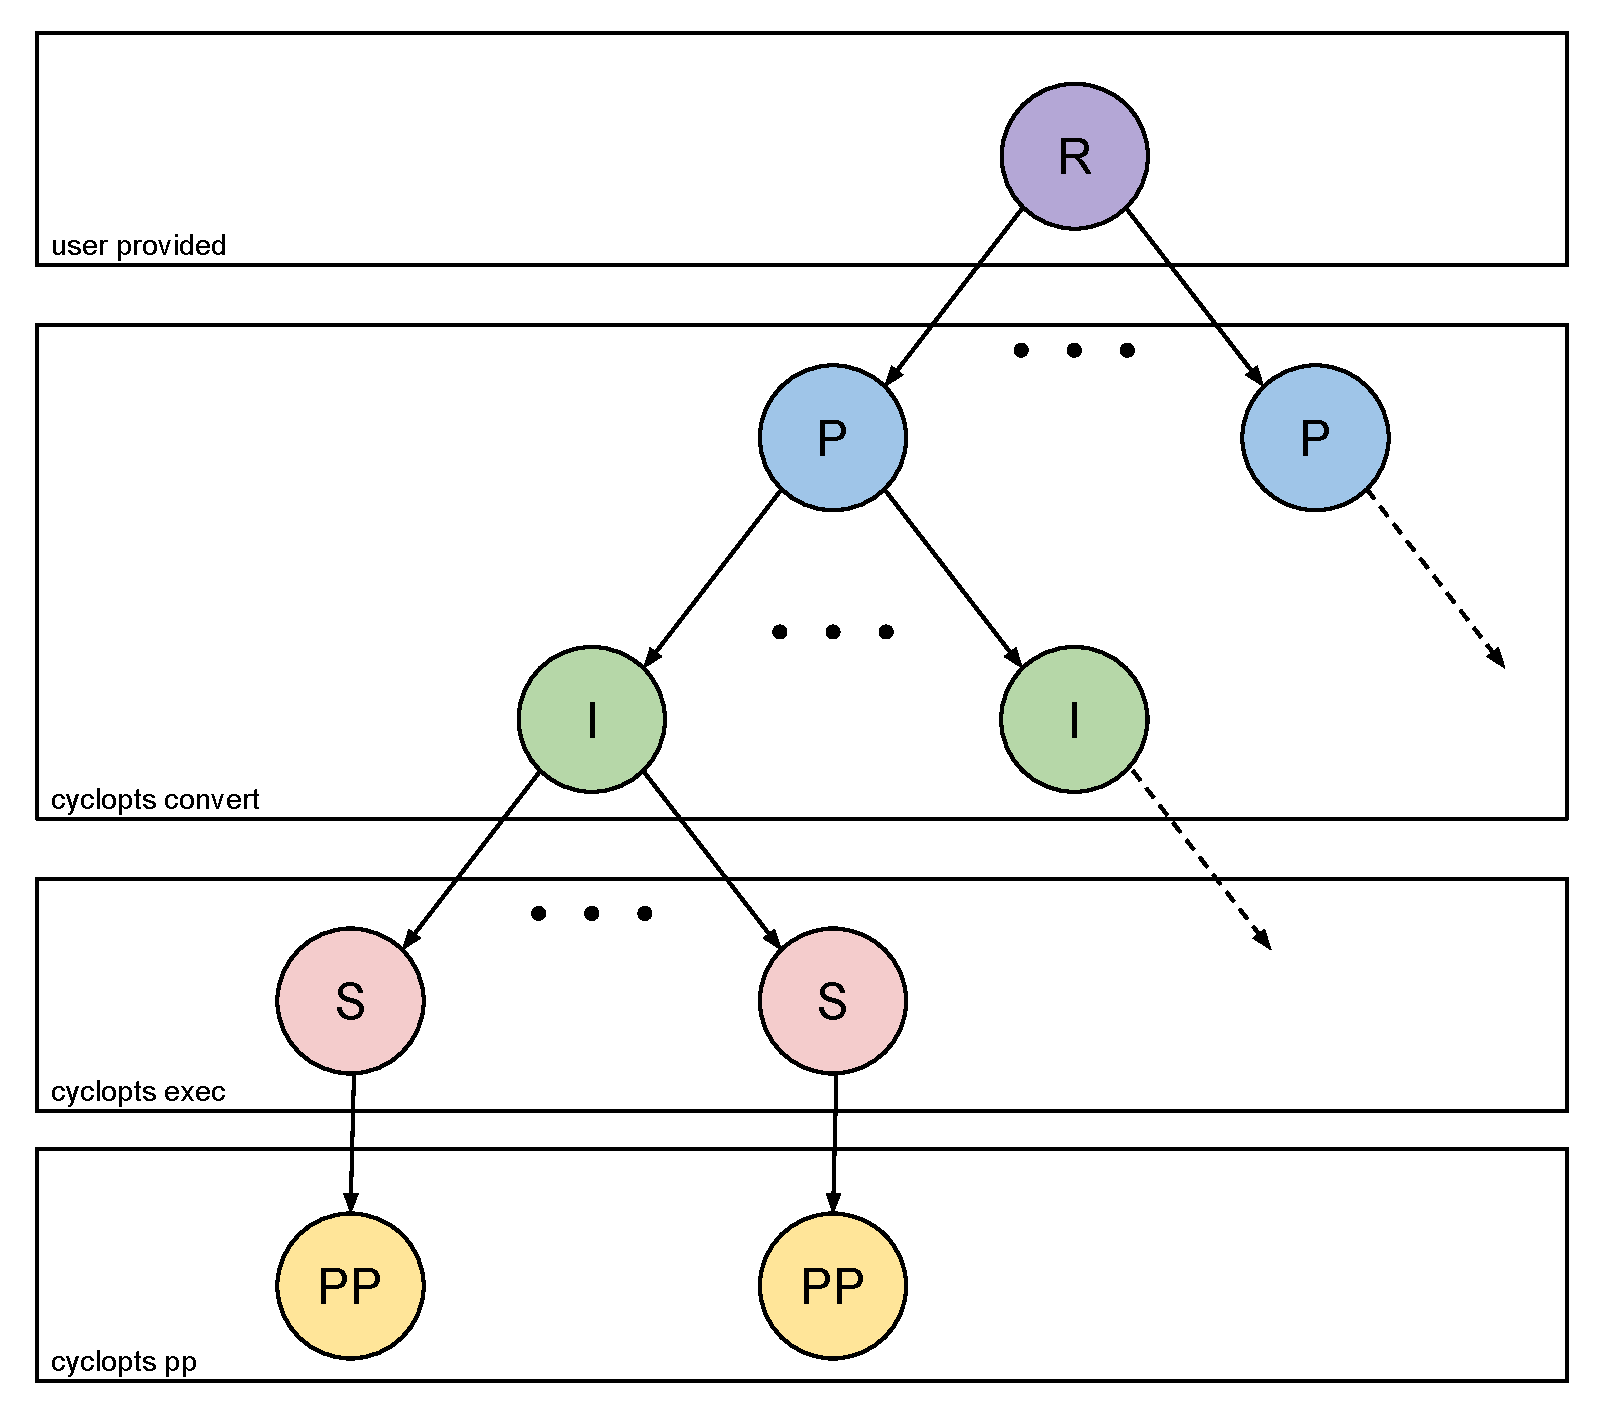
\includegraphics[width=\textwidth]{./backmatter/figs/cyclopts_tree_cli.pdf}
    \caption[]{
      \label{fig:lopts_cli}
      The Cyclopts object tree structure is shown with boxes around each group
      of objects that are created given a CLI call. Note that the root node is
      determined from user-provided input.}
  \end{center}
\end{figure}

\section{Remote Execution}

In order to execute Cyclopts on a Condor system, the submit node must contain
the Cyclopts environment. That operation is supported by the \code{cyclopts cde}
CLI, presented in Listing \ref{lst:loptscde}. A job, the input of which is an
instance database, can be submitted using \code{cyclopts condor-submit}. Upon
completion, results can be collected with \code{cyclopts condor-collect}. The
arguments for both are shown in Listings \ref{lst:loptscondor-submit} and
\ref{lst:loptscondor-collect}.

\lstinputlisting[
  style=BashOutputStyle,
  keywordstyle=\ttfamily,
  caption={CLI options for \code{cyclopts cde}.}, 
  label=lst:loptscde]{./backmatter/listings/cde}

\lstinputlisting[
  style=BashOutputStyle,
  keywordstyle=\ttfamily,
  caption={CLI options for \code{cyclopts condor-submit}.}, 
  label=lst:loptscondor-submit]{./backmatter/listings/condor-submit}

\lstinputlisting[
  style=BashOutputStyle,
  keywordstyle=\ttfamily,
  caption={CLI options for \code{cyclopts condor-collect}.}, 
  label=lst:loptscondor-collect]{./backmatter/listings/condor-collect}

\end{appendices}

%% McBride is a very nice style (some version is included in this distribution)
\bibliographystyle{mcbride}
\bibliography{./bibs/refs,./bibs/simulators,./bibs/benchmarks,./bibs/cosi,./bibs/abm-supply-chain,./bibs/blending}%,./chapters/litreview/refs}

%% Want an index?  Neither did I.
%\printindex

\end{document}
